\documentclass[usenames,dvipsnames,t]{beamer}
\usepackage[english]{babel}
\usepackage[utf8]{inputenc}
\usepackage{amsmath,amsthm, amssymb, latexsym}
\boldmath
\usepackage{color}
\usepackage{tikz}
\usepackage{standalone}
\usepackage{minted}
\usepackage{hyperref}
\usepackage{graphicx}
\usepackage{wrapfig}
\usepackage{rotating}
\usepackage{fontawesome}

\makeatletter
\setlength{\@fptop}{0pt}
\makeatother
\setlength{\columnsep}{2pt}

\definecolor{LightGray}{gray}{0.2}
\usemintedstyle{native}

\usetikzlibrary{decorations.pathmorphing}
\usetikzlibrary{fit}                    % fitting shapes to coordinates
\usetikzlibrary{backgrounds}    % drawing the background after the foreground

\tikzstyle{background}=[red!79, rectangle, draw, inner sep=-0.5mm,
           rounded corners=1mm, thick]

\usecolortheme[dark,accent=cyan]{solarized}
\beamertemplatenavigationsymbolsempty
\setbeamerfont{block title}{size=\Large}
\usepackage[orientation=landscape,size=a1,scale=1.4]{beamerposter}

%%%%%%%%%%%%%%%%%%%%%%%%%%%%%%%%%%%%%%%%%%%%%%%%%%%%%%%%%%%%%%%%%%%%%%%%%%%%%%%
\begin{document}
\begin{frame}[fragile]
\begin{columns}[t]
 \begin{column}{.53\linewidth}

  \Huge{\textcolor{solarizedRed}{SHOULD PEOPLE HOLD A GRUDGE?} \textcolor{OliveGreen}{WHAT IS}\\
  \textcolor{OliveGreen}{THE OPTIMAL PLAY IN A WAR?} \textcolor{cyan}{SOUTH AND}\\
  \textcolor{cyan}{NORTH JOIN HANDS TO DEFEAT THE NIGHT
  KING?}}
  %   \end{block}
  \end{column}
  \begin{column}{.22\linewidth}
 
  \Large{\textcolor{brown}{GAME THEORY} IS THE STUDY OF STRATEGY INTERACTIONS. THE \textcolor{brown}{PRISONERS DILEMMA} IS A GAME USED TO UNDERSTAND THE EVOLUTION OF CO- OPERATIVE BEHAVIOUR.}
  \end{column}
  \begin{column}{.20\linewidth}

  \includestandalone[width=1\textwidth]{static/matrix}
  \end{column}
  \end{columns}
  \begin{columns}[t]
    \begin{column}{.30\linewidth}

    \hspace{3cm}

    % \textcolor{brown}{\Large{\textbf{HOW IT WAS DONE?}}} \\
    % \Large{The Axelrod Python Library has more than \textcolor{brown}{200 condtibutors}, \textcolor{brown}{100\%} test coverage, unit and integration 
    % \textcolor{brown}{testing} and is well \textcolor{brown}{documented}}.
\includestandalone[width=\textwidth]{static/match}

\noindent\rule[0.5ex]{\linewidth}{1pt}
    \begin{minted}
    [
    autogobble=true,          % Automatically remove common whitespace
    %bgcolor=dark-bg,
    frame=lines,
    framesep=2mm,
    fontsize=\normalsize
    ]
    {python}
import axelrod as axl

first_match = axl.Match([axl.TitForTat(), 
                         axl.SneakyTitForTat()])
second_match = axl.Match([axl.Grudger(), 
                          axl.SneakyTitForTat()])

play = first_match.play()
first_match.final_score()
(297, 297)

play = second_match.play()
second_match.final_score()
(295, 60)
    \end{minted}
\Large{Assume a colice of your is forgetful and Defcts againsts. SHould a person hold a grudge or should let their collide retailete? The Axelrod Python library allow you to create a match between a 'Sneaky' player and allow us
to compare the results of two diffrent actions of ours.}

\hspace{10cm}
\noindent\rule[0.5ex]{\linewidth}{1pt}

\large{\textbf{MORE INFORMANTION}}
          \begin{itemize}
          \item In case you missed me:
          \item Github: \url{https://github.com/Axelrod-Python}
          \end{itemize}

\hspace{1cm}

\large{\textbf{ABOUT ME}}
\hspace{1cm}

\faTwitter \large{ NikoletaGlyn} \\
\faGithub \large{ Nikoleta-v3}
      \end{column}
    \begin{column}{.30\linewidth}

      \Large{In a game of war several players collide. The players interact 
      with the rest players and that's when a question rises: \\
      \begin{center}\textcolor{OliveGreen}{`What is a player's optimal strategy?'}\end{center}}

    \begin{columns}
    \begin{column}{.60\linewidth}
    \large{The Axelrod Python Library allows us to create different 
    enviroments, \textcolor{OliveGreen}{tournaments}, and choose from over 200 different strategic plays. This allow us to explore different possible war scenarios and winners.}
    \end{column}
    \begin{column}{.40\linewidth}
    \begin{center}
    \includestandalone[width=0.8\textwidth]{static/tournament}
    \end{center}
    \end{column}
    \end{columns}

    \begin{center}
    \begin{minted}
    [
    autogobble=true,          % Automatically remove common whitespace
    %bgcolor=dark-bg,
    frame=lines,
    framesep=2mm,
    fontsize=\normalsize
    ]
    {python}
import axelrod as axl

axl.seed(0)
players = [axl.Cooperator(), axl.Defector(), 
           axl.TitForTat(), axl.Grudger(), 
           axl.Random()]
tournament = axl.Tournament(players)
results = tournament.play()
results.ranked_names
['Defector', 'Grudger', 'Tit For Tat', 
 'Cooperator', 'Random: 0.5']

plot = axl.Plot(results)
p = plot.boxplot()
p.show()
    \end{minted}
    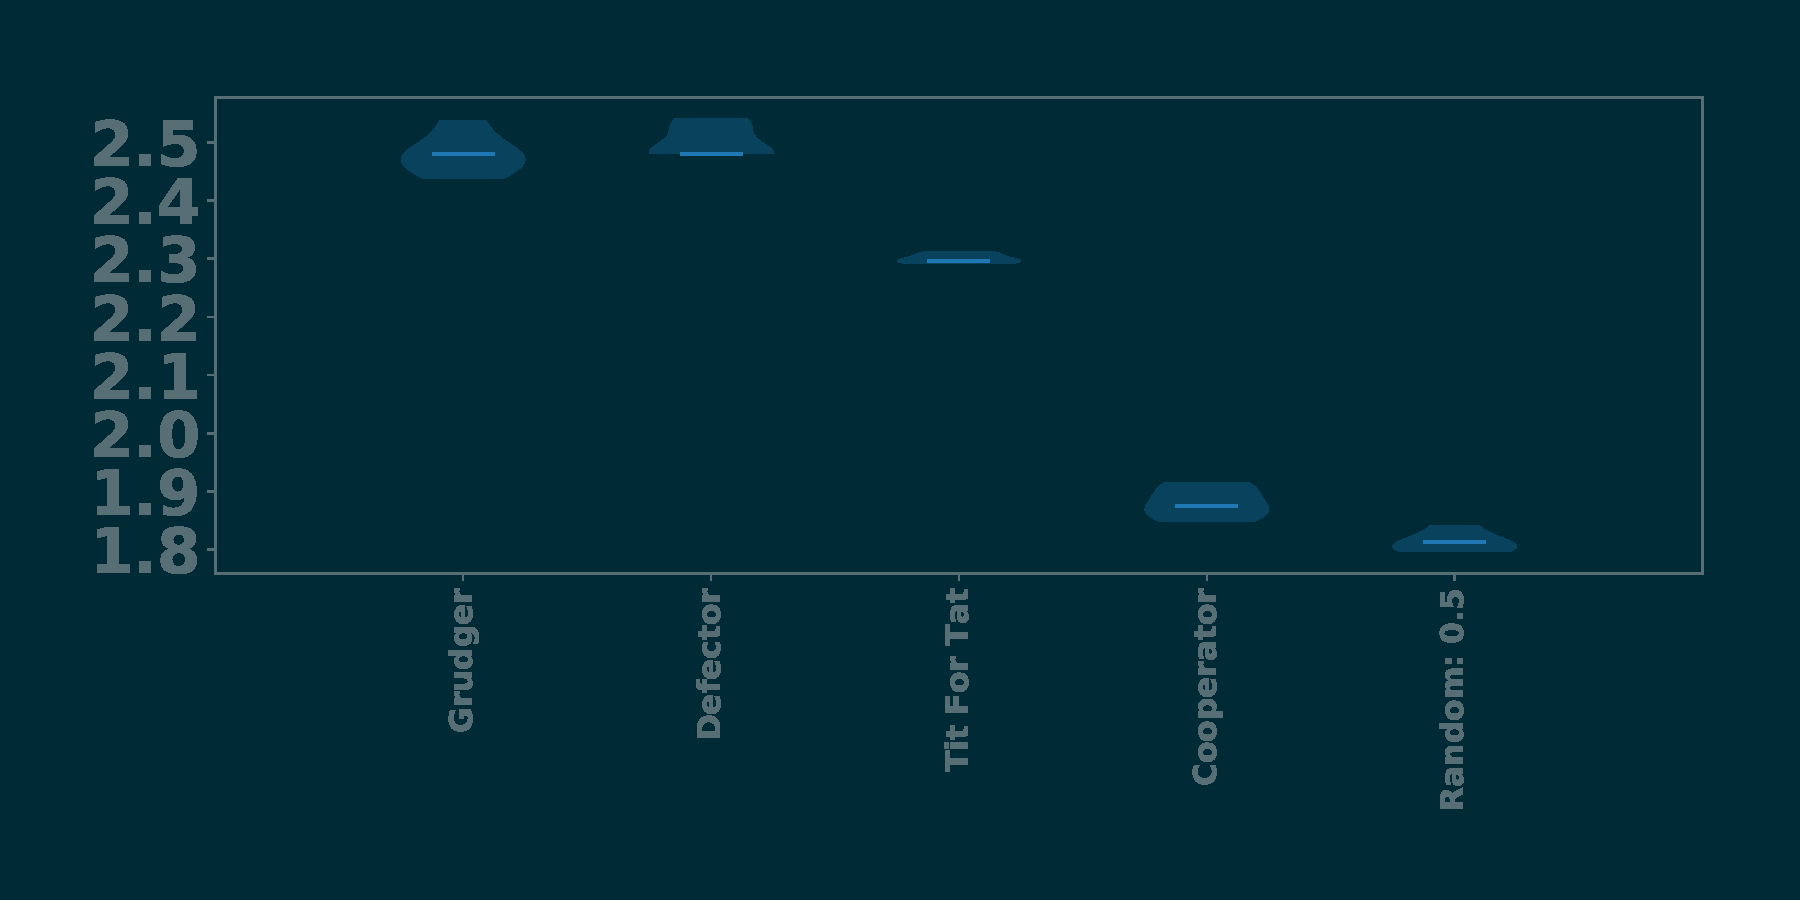
\includegraphics[width=\textwidth, height=0.55\textwidth]{static/tournament_results.pdf}
    \end{center}
  \end{column}
      \begin{column}{.30\linewidth}

        \begin{center}
        \includestandalone[width=0.8\textwidth]{static/evolution}
        \end{center}
        \Large{Following the recent events of Game of Thrones season 7 many 
        have wondered as to if the South and the North should work together
        against the army of the dead. More speficically should our players 
        cooperative or defect. \textcolor{cyan}{Evolutionary Game Theory} 
        allow us to study the evolution of such populations.}
    \begin{center}
    \begin{minted}
    [
    autogobble=true,          % Automatically remove common whitespace
    %bgcolor=dark-bg,
    frame=lines,
    framesep=2mm,
    fontsize=\normalsize
    ]
    {python}
N = 20
players = []
for _ in range(N):
    player = random.choice([axl.Defector, axl.Cooperator])
    players.append(player())

mp = axl.MoranProcess(players=players, turns=200)
mp.play()
[Counter({'Cooperator': 11, 'Defector': 9}),
 Counter({'Cooperator': 10, 'Defector': 10}),
          ......................
 Counter({'Cooperator': 1, 'Defector': 19}),
 Counter({'Defector': 20})]
    \end{minted}
    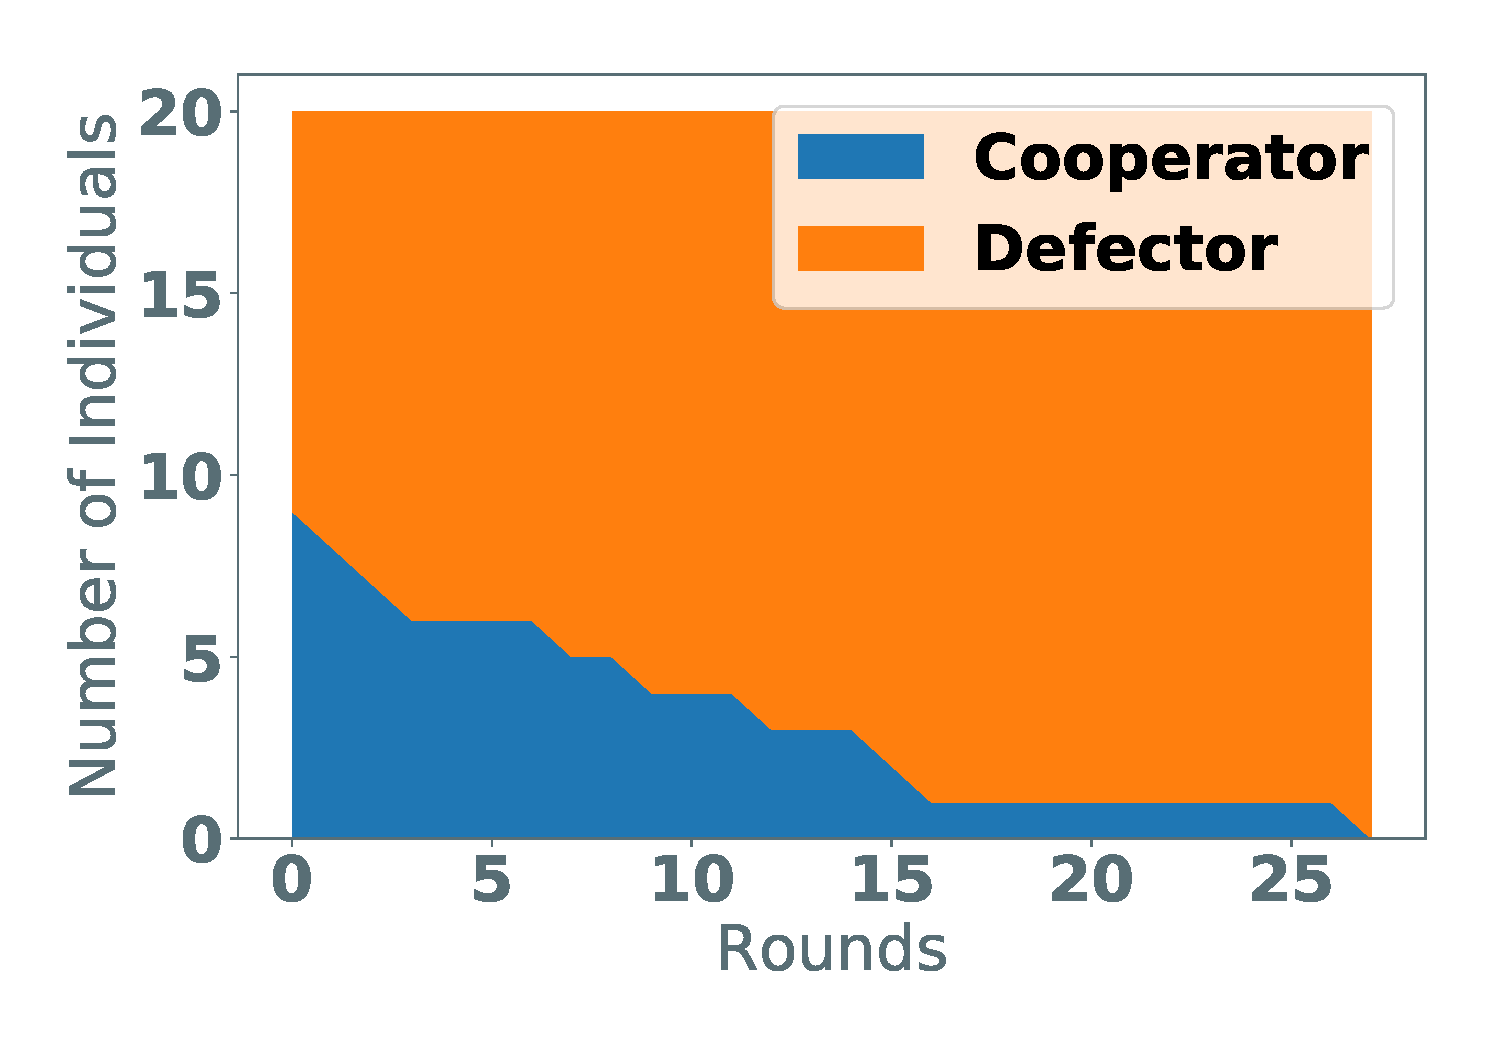
\includegraphics[width=0.8\textwidth, height=0.6\textwidth]{static/evolution.pdf}
    \end{center}

    \end{column}
    \end{columns}
\end{frame}
\end{document}

 
